\documentclass[]{article}

\usepackage{graphicx}
\graphicspath{ {Pictures/} }

% Title Page
\title{Getting started with \linebreak Husqvarna Research Platform}
\author{Fredrik B\aa berg \\ \small{Computer Vision and Active Perception} \\ \small{KTH} }
\date{January 2016}


\begin{document}
\maketitle

\begin{abstract}
This document explains how to setup the Husqvarna Research Platform on a computer. It details the step of powering up the robot, starting simulation, and launching the teleoperation node.
\end{abstract}

\begin{figure}[h]
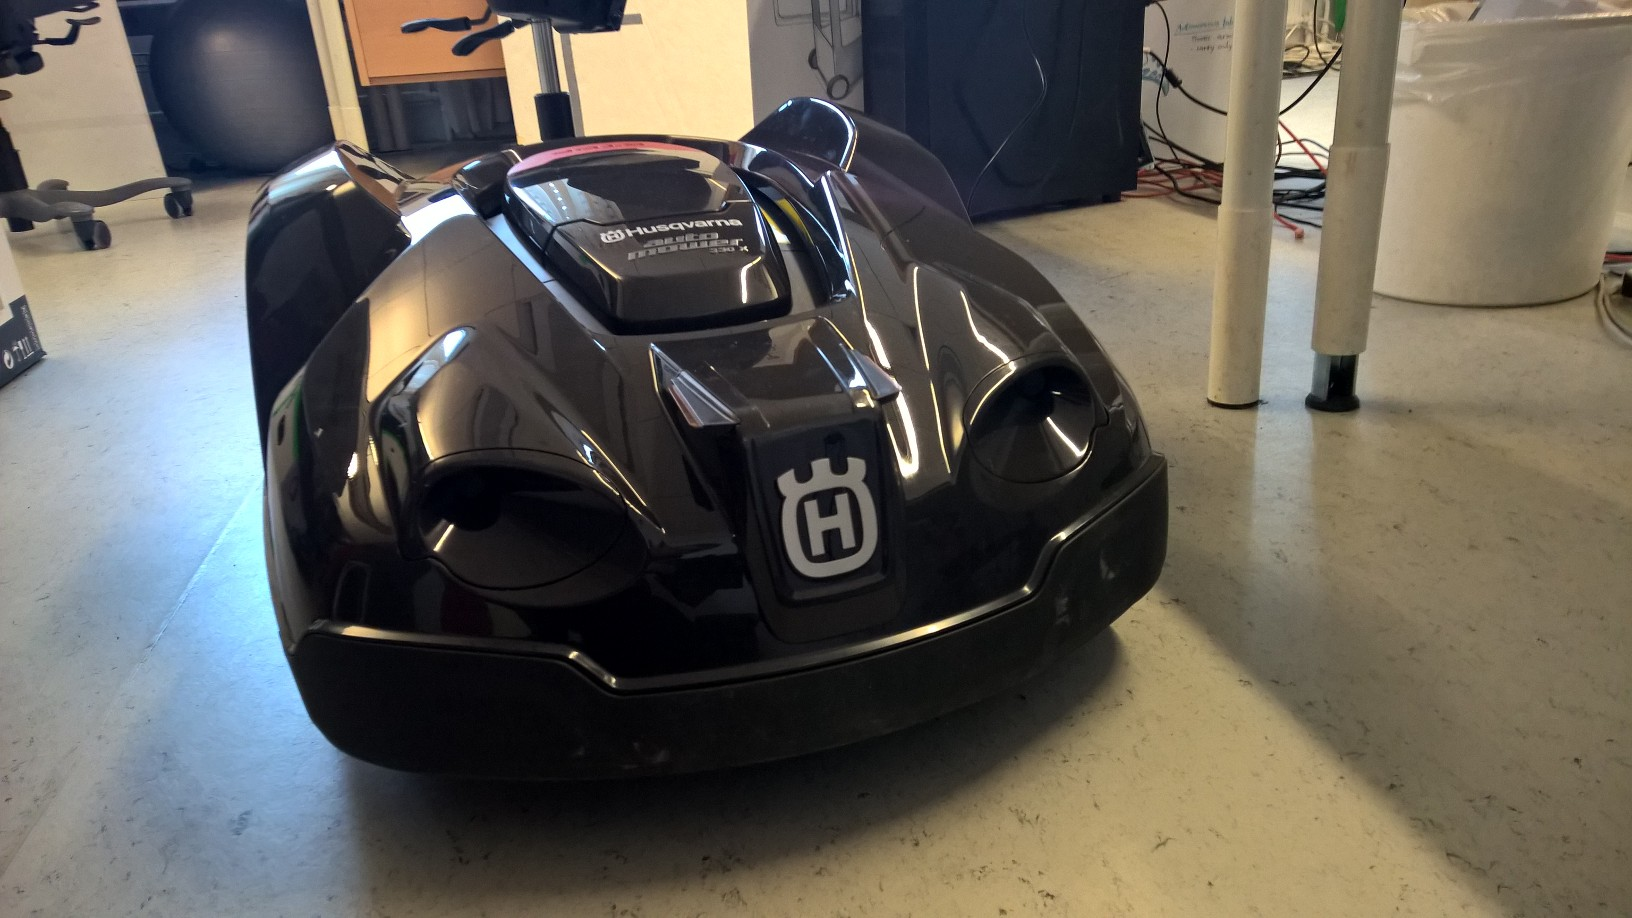
\includegraphics[width=12cm]{hrp.jpg}
\centering
\end{figure}

\section{Installation}
This section describes how to install software needed.

\subsection{Install software on PC}\label{sec:install_pc}
This document assumes all code will be located in a catkin workspace src folder, in this case \verb|~/ws/src/|. Extract the archive through \verb|tar -xvf hrp*|, where \verb|hrp*| indicates the tar.gz archive.
\begin{itemize}
\item Install some additional packages that will be needed:
\begin{verbatim}
sudo apt-get install ros-indigo-nmea-msgs libcgal-dev screen
\end{verbatim}
\item Also need to install dependencies from catkin workspace. It is possible \verb|catkin_make| has to be executed first:
\begin{verbatim}
cd ~/ws
catkin_make
rosdep install --from-paths src --ignore-src --rosdistro indigo
\end{verbatim}
\end{itemize}
Now build the workspace through \verb|catkin_make|. Don't forget to source the workspace \verb|source ~/ws/devel/setup.bash|, it could be useful to add this to \verb|~/.bashrc|

\subsection{Preparation for running on hardware}\label{sec:install_hardware}
An additional installation step is needed for running on hardware, related to communication with the robot. This step is a preparation that should only be needed once on the device.
\begin{itemize}
\item Add the current user to the \verb|dialout| group through the command
\begin{verbatim}
sudo adduser <username> dialout
\end{verbatim}
\end{itemize}
You will need to log out and log in before you continue.

\section{Running}\label{sec:run}
With everything installed, you are now almost ready for launch.

\subsection{Start robot}\label{sec:run_robot}
To prepare the robot for usage in a lab environment (without using a \textit{loop}, other word for the wire), follow this procedure:
\begin{itemize}
\item Change power switch to \textbf{ON}
\item Enter PIN code (\textbf{1111})
\item Press \textbf{MENU}
\item Hold 7 and 9 until new menu (\textbf{TOOLS}) appears
\item Select wrench, press \textbf{OK}
\item Select \textbf{Special settings} (last entry in list), press \textbf{OK}
\item Tick \textbf{Override loop detection} by pressing \textbf{OK}
\item Press \textbf{OK} to confirm
\item Press \textbf{START}, or \textbf{BACK} until start menu appears and then \textbf{START}
\item Close hatch (or use plastic switch), display should now say \textbf{MOWING}, the platform will move slightly, and is then ready for use
\end{itemize}

\subsection{Start Gazebo}\label{sec:run_gazebo}
For using Gazebo, one additional step is required. It could be useful to add this line to your \verb|~/.bashrc| file, to avoid typing it every time
\begin{verbatim}
export GAZEBO_MODEL_PATH=~/ws/src/hrp/am_gazebo/models:$GAZEBO_MODEL_PATH
\end{verbatim}

Gazebo, together with robot and an environment, can then be launched through
\begin{verbatim}
roslaunch am_gazebo am_gazebo_hrp_tracking.launch gui:=true
\end{verbatim}
Note that there are several parameters that could be set, look in the launch file. When launching both Gazebo and running on hardware, it could be useful to add \verb|app:=false steering:=false| so that the robot doesn't automatically move on launch.

\subsection{Launch hardware drivers}
Before launching, make sure you have the correct port. Start the platform according to Section \ref{sec:run_robot}, and connect the USB cable.
\begin{itemize}
\item Check which port is used through \verb|dmesg|, it could for instance be \verb|/dev/ttyACM0| (0 is the number zero)
\begin{verbatim}
dmesg | grep ACM
\end{verbatim}

\item Now update the device through the following command, assuming that the device you got was \verb|ttyACM0|:
\begin{verbatim}
screen /dev/ttyACM0 115200
\end{verbatim}

\item The terminal will now be blank. Press \verb|ctrl+a| followed by \verb|k| and \verb|y| to kill screen.
\end{itemize} 

The steps before should only be needed once. To run the drivers, make sure \verb|roscore| is running, and execute \verb|rosrun am_driver am_driver_node| to run the driver. Output should end with
\begin{verbatim}
Serial port ONLINE!
Serial port connected!
\end{verbatim}
if everything is correct.

\subsection{Teleoperation}\label{sec:run_teleop}
To launch the teleoperation node, execute the following
\begin{verbatim}
rosrun am_control key_teleop.py
\end{verbatim}
You can switch between teleoperation and random behavior through \textbf{1} and \textbf{2}. For other commands, see the python script.

\subsection{UWB sensors}
To launch the UWB sensors, connect the master \textbf{s100} to the computer using an FTDI cable (3.3V), and check which USB port is used (could be \verb|/dev/ttyUSB0|). Launch through
\begin{verbatim}
rosrun am_uwbrange am_uwbrange_node _serialPort:=/dev/ttyUSB0
\end{verbatim}
Information is then published on ROS topic \verb|/uwb|. It will include range between all sensors found.
\begin{figure}[h]
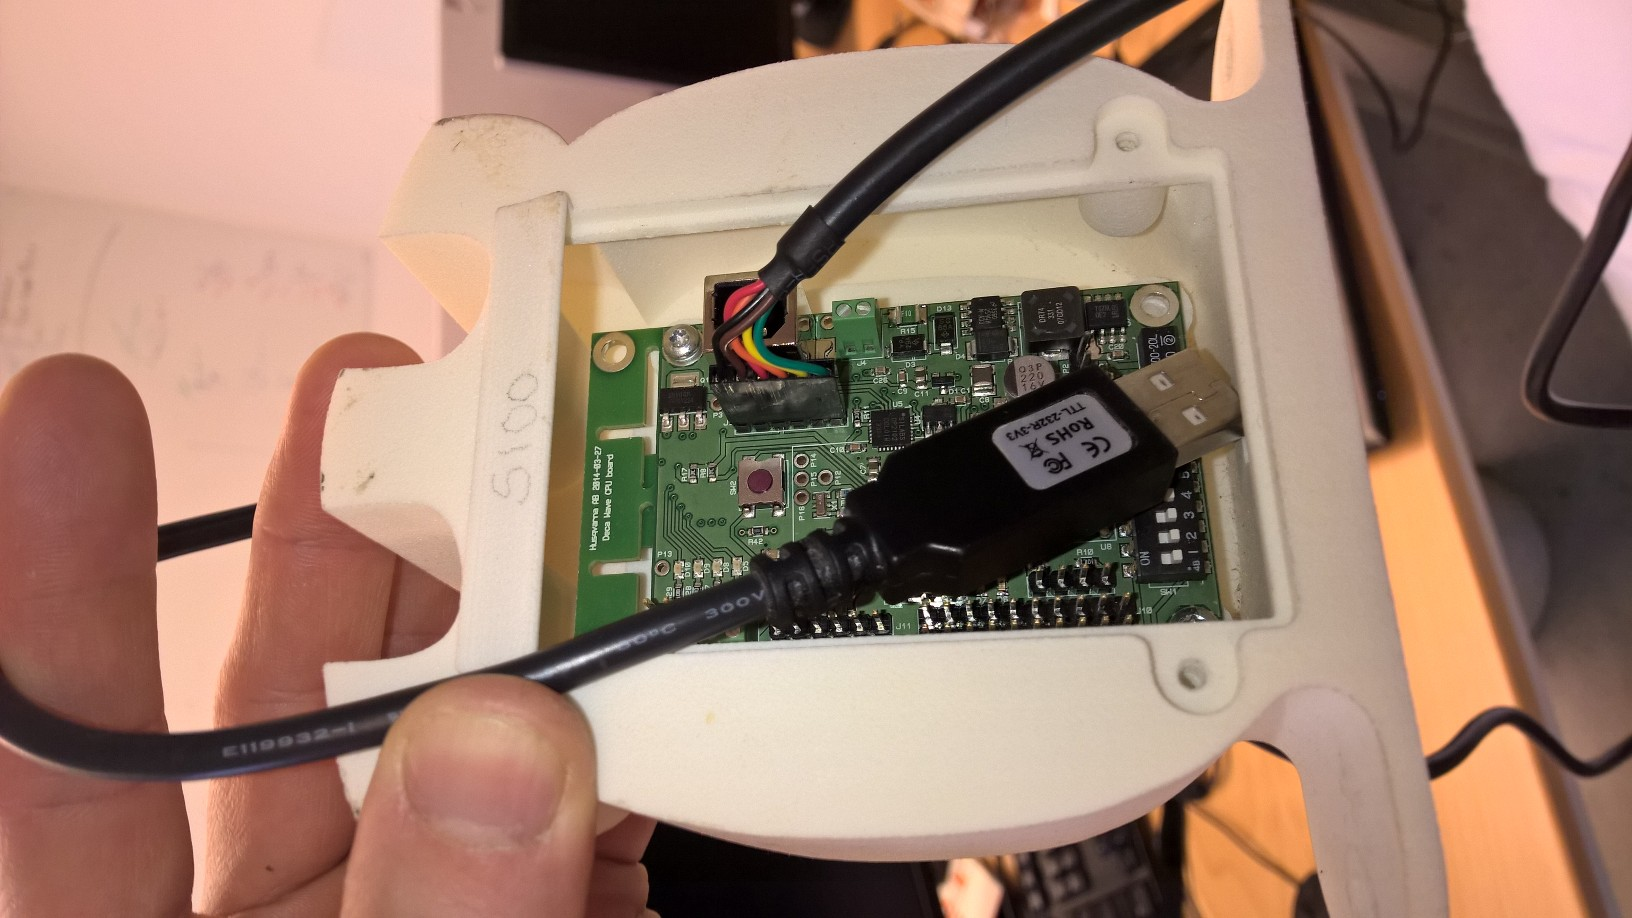
\includegraphics[width=8cm, angle=270]{uwb.jpg}
\centering
\caption{Connection of FTDI cable, with ground visible}
\end{figure}

\end{document}          
